\chapter{Specific Requirements} \label{specificRequirements}
\section{External Interfaces}
\begin{itemize}
  \item \textbf{Web Application Interface:} Handles user interactions with the FarmBot via a web platform. Functions include user authentication, data retrieval (such as sensor and hardware information), displaying resource usage, system information, and scheduling tasks on the FarmBot.
  \item \textbf{User Interface:} Direct interface for the user to interact with FarmBot's functions. It includes personal identification details and commands for various farming operations like watering, planting, fertilizing, and harvesting.
  \item \textbf{System Admin Interface:} Tailored for administrators to maintain the FarmBot system, providing access to system configurations, user management, and oversight of operational logs and updates.
  \item \textbf{OpenFarm.cc API:} Connects with the OpenFarm database, offering users extensive crop data and farming knowledge exchange.
\end{itemize}
Each interface serves a distinct role, ensuring the FarmBot ecosystem is accessible and manageable by different stakeholders, from end-users to developers and community contributors.

\begin{figure}[htbp]
        \centering
        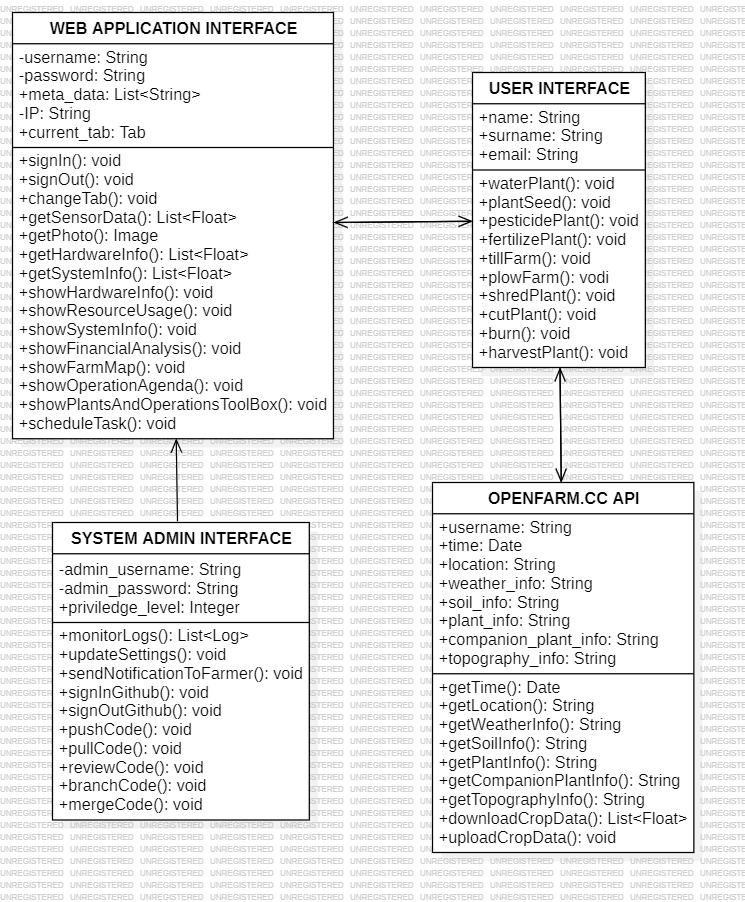
\includegraphics[width=1\linewidth]{Figures/external_interfaces.jpg}
        \caption{External Interfaces}
        \label{ExternalInterfaces}
\end{figure}

\newpage

\section{Functions}
The use case diagram showcases ten distinct scenarios, including four actors. On the diagram's left-hand side, the primary actors, namely the user and system admin, are positioned, while on the right-hand side, the secondary actors, which include the Web Application and OpenFarm.cc API, are positioned. The use case diagrams are supported with description tables. Additionally, the use cases titled "Control Hardware," "Monitor Farm Data," and "Store Farm Data" are further explained using an activity diagram, a sequence diagram, and a state diagram, respectively.\\

% Use Case Diagram
\begin{figure}[htbp]
        \centering
        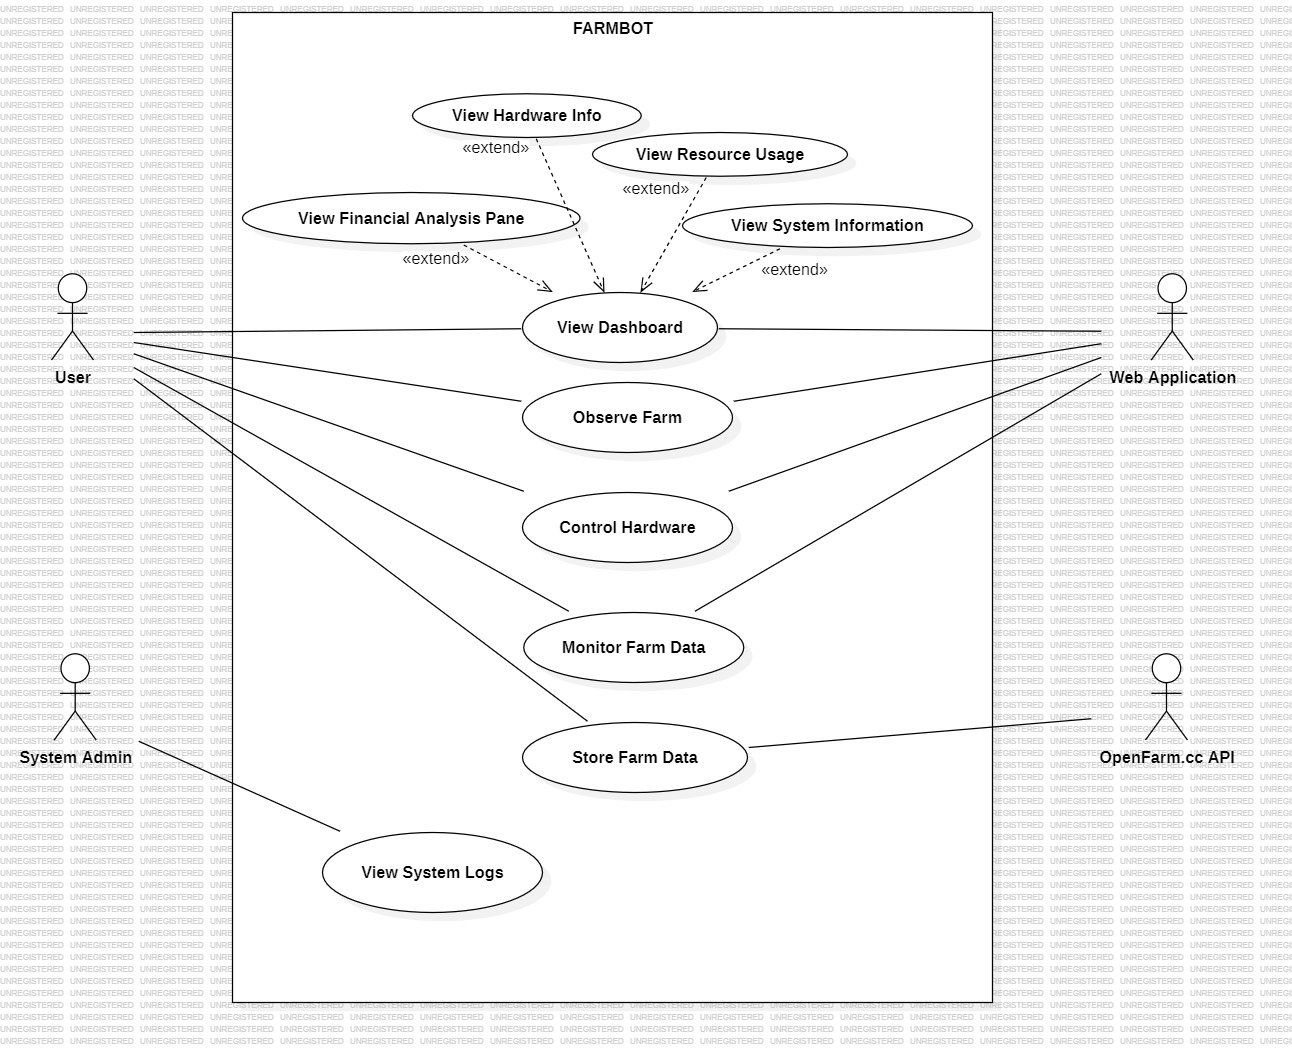
\includegraphics[width=1\linewidth]{Figures/use_case_diagram.jpg}
        \caption{Use Case Diagram}
        \label{UseCaseDiagram}
\end{figure}

\newpage

% View Dashboard Use Case Table
\begin{longtblr}
[
 caption = {Tabular Description of the \textbf{View Dashboard} Use Case},
 label = {ViewDashboard}
]
{
  colspec = {|X|X|},
  hlines
}
\textbf{Use Case Name} & View Dashboard \\ \hline
\textbf{Actors} & User, Web Application \\ \hline
\textbf{Description} & The user views the dashboard containing various information from his/her farm. \\ \hline
\textbf{Preconditions} & The user must be logged into the FarmBot Web Application. \\ \hline
\textbf{Data} & System, Resource, Hardware, and Financial information and data obtained from the sensors of FarmBot \\ \hline
\textbf{Response} & A GUI facilitating control and analysis of the Farm. \\ \hline
\textbf{Stimulus} & The user selects the "Dashboard" option within the Web Application. \\ \hline
\textbf{Normal Flow} & {
	1. The user is directed to the dashboard pane on button click.\\
	2.  If s/he is already logged into the site, the system automatically sends a signal to the FarmBot device to obtain the necessary information.\\
	3. FarmBot sends the data obtained from the various sensors to the Web Application in order to be displayed on the dashboard tab.\\
	4. While the user is dragging the graph about resources, the new data corresponding to the point to where the user dragged graph is obtained by the sensors.\\
	5. If the user uses the manual control tab, the web application sends a signal to the hardware to move.
}
\\ \hline
\textbf{Alternative Flow} & - \\ \hline
\textbf{Exception Flow} & If the user is not logged into the site, or his/her session has expired, s/he is automatically directed to the login page.  \\ \hline
\textbf{Post Conditions} & The dashboard tab must be displayed on the screen. \\ \hline
\textbf{Comments} & Sending localized data offers a more smooth experience to users since it reduces the loading time of the graphs. Moreover, calculating the session time and checking for the user authentication improves the security of the application.
\end{longtblr}

% Observe Farm Use Case Table
\begin{longtblr}
[
 caption = {Tabular Description of the \textbf{Observe Farm} Use Case},
 label = {ObserveFarm}
]
{
  colspec = {|X|X|},
  hlines
}
\textbf{Use Case Name} & Observe Farm \\ \hline
\textbf{Actors} & User, Web Application \\ \hline
\textbf{Description} & The user observes his/her farm thanks to the camera integrated to the FarmBot. \\ \hline
\textbf{Preconditions} & The user must be logged into the FarmBot Web Application. \\ \hline
\textbf{Data} & Images and visual data from the farm captured by the camera. \\ \hline
\textbf{Response} &  The Web Application displays the latest farm images and data, allowing for visual analysis. \\ \hline
\textbf{Stimulus} & The user selects the "Farm" option within the Web Application. \\ \hline
\textbf{Normal Flow} & {
	1. User selects "Observe Farm" from the Web Application.\\
	2. The system verifies that the user is logged in.\\
	3. The Web Application sends a request to the FarmBot to capture current farm images.\\
	4. The camera captures images and sends them to the Raspberry Pi.\\
	5. The Raspberry Pi processes and uploads the images to the Web Application.\\
	6. The Web Application displays the images to the user for observation.
}
\\ \hline
\textbf{Alternative Flow} & - \\ \hline
\textbf{Exception Flow} &  If the user is not logged in, or the session has expired, they are redirected to the login page. \\ \hline
\textbf{Post Conditions} & The user is able to visually inspect the farm through the latest images displayed on the Web Application. \\ \hline
\textbf{Comments} & Providing real-time or regularly updated images allows users to closely monitor their farm's condition without needing to be physically present. This feature enhances the overall user experience by facilitating remote farm management and decision-making.
\end{longtblr}

% Control Hardware Use Case Table
\begin{longtblr}
[
 caption = {Tabular Description of the \textbf{Control Hardware} Use Case},
 label = {Control Hardware}
]
{
  colspec = {|X|X|},
  hlines
}
\textbf{Use Case Name} & Control Hardware \\ \hline
\textbf{Actors} & User, Web Application \\ \hline
\textbf{Description} & Users send commands to control FarmBot's hardware via the Web Application. \\ \hline
\textbf{Preconditions} & The user must be logged into the FarmBot Web Application and the FarmBot hardware must be operational and connected to the internet. \\ \hline
\textbf{Data} & Command inputs for hardware operation (e.g., watering, moving, planting). \\ \hline
\textbf{Response} & The hardware executes the specified operations and provides feedback on the action taken. \\ \hline
\textbf{Stimulus} & The user inputs hardware control commands through the dashboard and farm pane. \\ \hline
\textbf{Normal Flow} & {
	1. User navigates to the dashboard pane.\\
	2. User selects the desired tools and hardware to control (e.g., move the gantry or cross slide, water a specific area).\\
  3. User gives commands.\\
	4. The Web Application sends the command to Raspberry Pi.\\
	5. Raspberry Pi executes the command and sends a completion signal back to the Web Application.\\
	6. The Web Application displays a confirmation or result of the executed command to the user.
}
\\ \hline
\textbf{Alternative Flow} & {
  1. User sets a new schedule and chooses the hardware operations to automate (e.g., watering every morning at 7 AM, seeding specific areas on specific dates).\\
  2. User sets the specific timing and frequency for each operation, along with any necessary parameters (e.g., water volume, seed type).\\
  3. The Web Application saves the schedule and automatically sends commands to the FarmBot hardware based on the defined schedule.\\
  4. At the scheduled times, FarmBot executes the pre-defined operations without the need for real-time user input.\\
  5. After each scheduled operation, FarmBot sends a completion signal back to the Web Application.
}
\\ \hline
\textbf{Exception Flow} & If the hardware is unreachable or an error occurs during operation, an error message is displayed. \\ \hline
\textbf{Post Conditions} & The specified hardware operation is completed, and the user is informed of the outcome. \\ \hline
\textbf{Comments} & This use case is crucial for remote management of the FarmBot, allowing users to interact with their farm in real-time. Error handling and feedback mechanisms are essential for a smooth user experience and for troubleshooting purposes.
\end{longtblr}

% Control Hardware Activity Diagram
\begin{figure}[htbp]
  \centering
  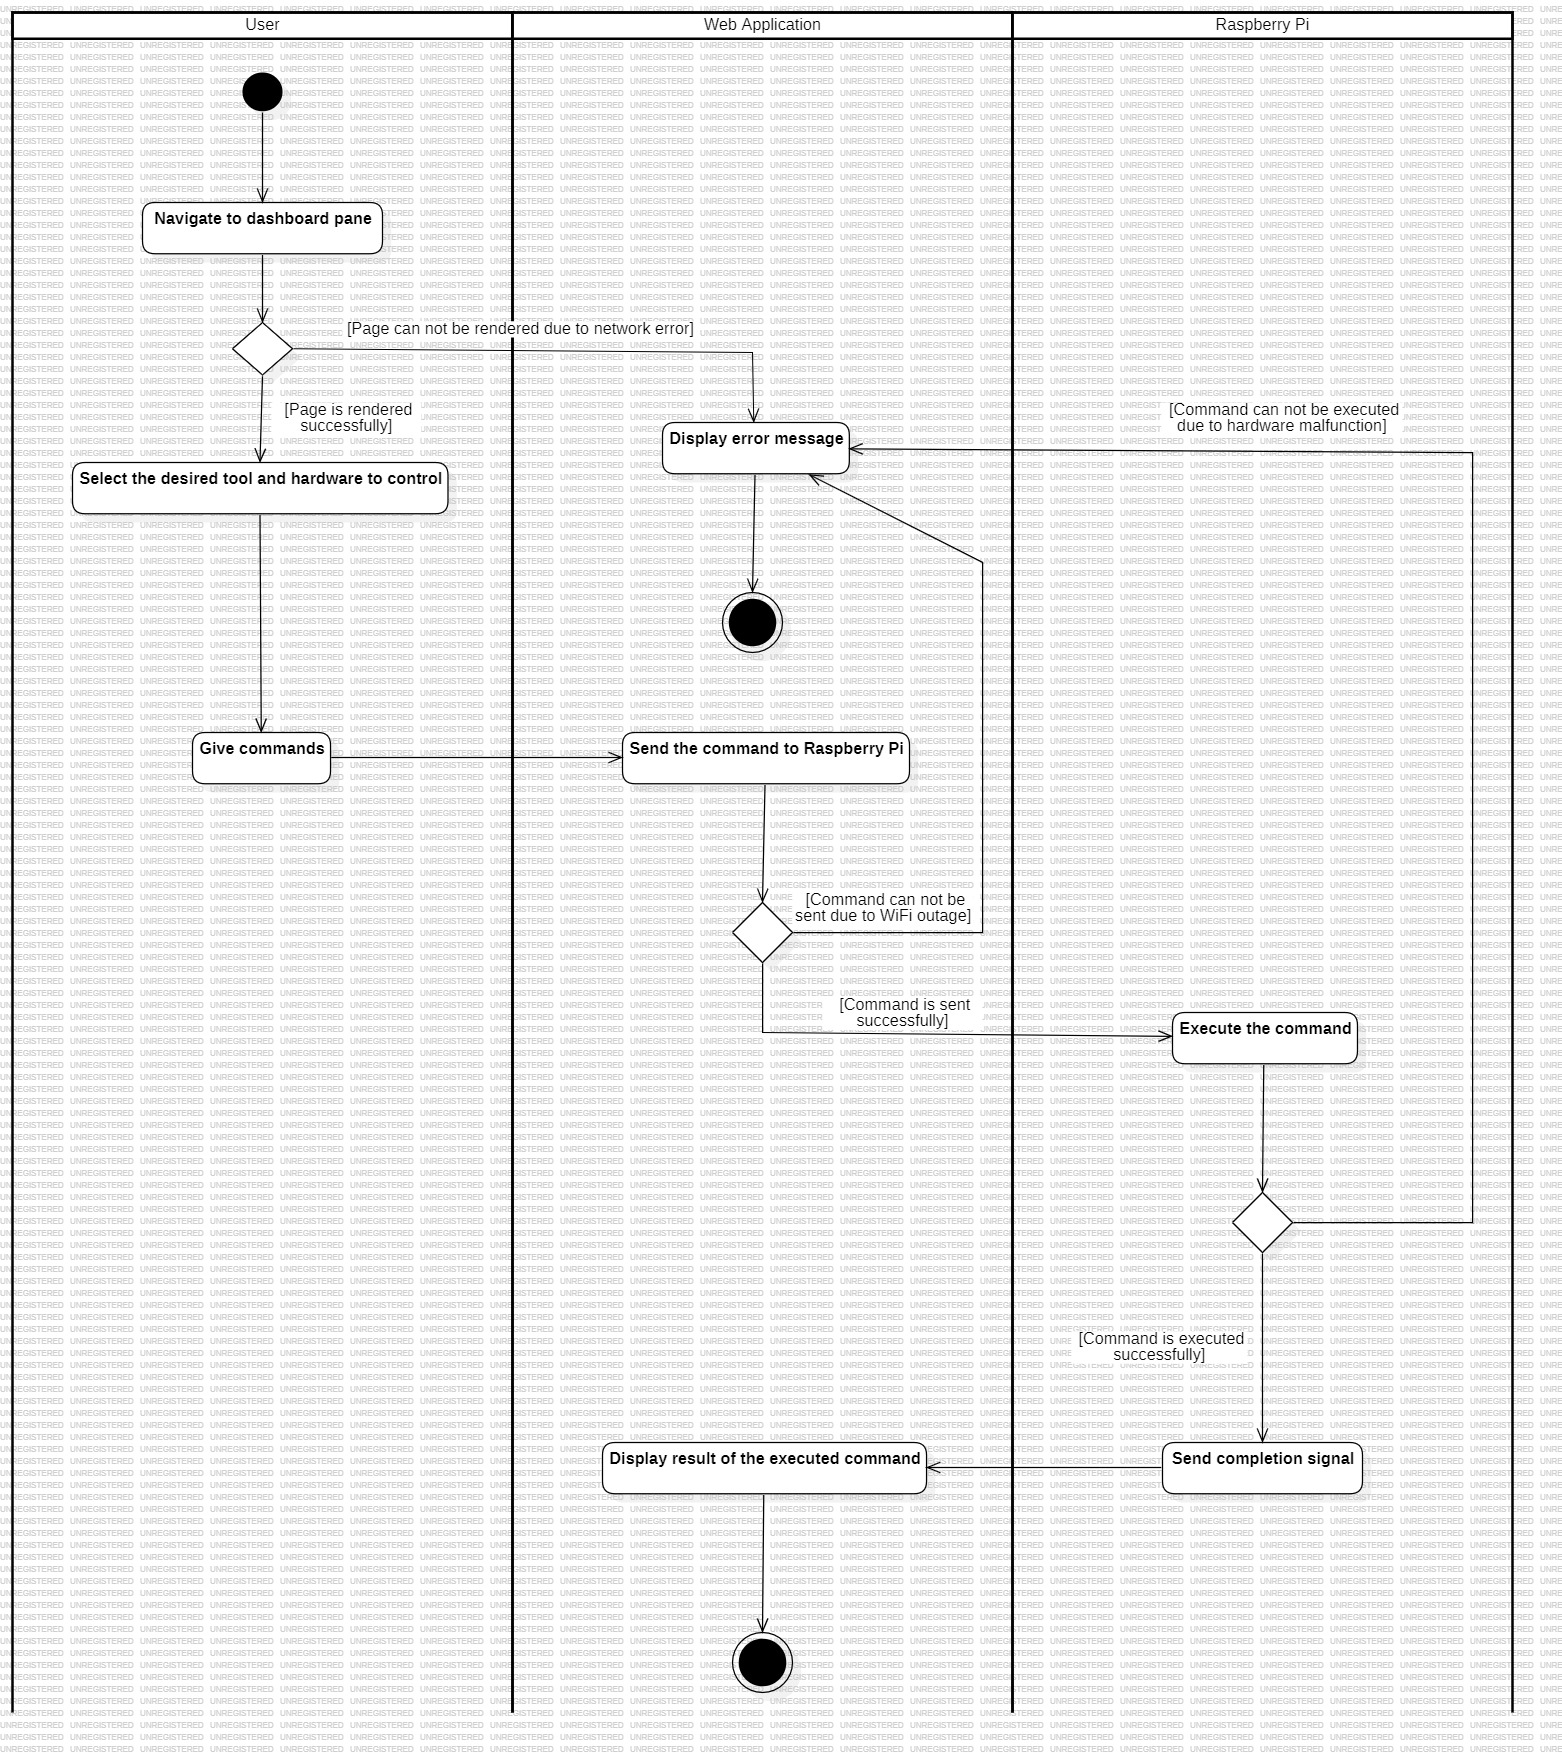
\includegraphics[width=1\linewidth]{Figures/control_hardware_activity_diagram.jpg}
  \caption{Activity Diagram for \textbf{Control Hardware} Use Case}
  \label{ActivityDiagram}
\end{figure}

\newpage

% Monitor Farm Data Use Case Table
\begin{longtblr}
[
 caption = {Tabular Description of the \textbf{Monitor Farm Data} Use Case},
 label = {MonitorFarmData}
]
{
  colspec = {|X|X|},
  hlines
}
\textbf{Use Case Name} & Monitor Farm Data \\ \hline
\textbf{Actors} & User, Web Application \\ \hline
\textbf{Description} & Users access and review real-time and historical data collected by FarmBot's sensors and obtained from the Internet to monitor farm conditions. \\ \hline
\textbf{Preconditions} & The user must be logged into the FarmBot Web Application. FarmBot's sensors must be operational and collecting data. \\ \hline
\textbf{Data} & Sensor data including soil moisture, temperature, pH levels, and plant growth. \\ \hline
\textbf{Response} & The hardware executes the specified operations and provides feedback on the action taken. \\ \hline
\textbf{Stimulus} & The user inputs hardware control commands through the dashboard and farm pane. \\ \hline
\textbf{Normal Flow} & {
	1. User logs into the Web Application and navigates to the data section.\\
	2. The Web Application queries the latest sensor data from Raspberry Pi.\\
	3. FarmBot sensors transmit the requested data to the Raspberry Pi.\\
	4. The Raspberry Pi processes and sends data to the Web Application.\\
	5. The Web Application presents data to the user, including historical trends and real-time information.
}
\\ \hline
\textbf{Alternative Flow} & - \\ \hline
\textbf{Exception Flow} & If sensor data is not available due to hardware issues, an error message is displayed. \\ \hline
\textbf{Post Conditions} & The user has accessed and reviewed the farm's sensor and other users' data, enabling monitoring and decision-making for farm management. \\ \hline
\textbf{Comments} & Monitoring farm data is essential for effective farm management, allowing users to adjust practices based on environmental conditions and plant needs. This use case facilitates proactive and responsive farm care, enhancing productivity and sustainability.
\end{longtblr}

% Monitor Farm Data Sequence Diagram
\begin{figure}[htbp]
        \centering
        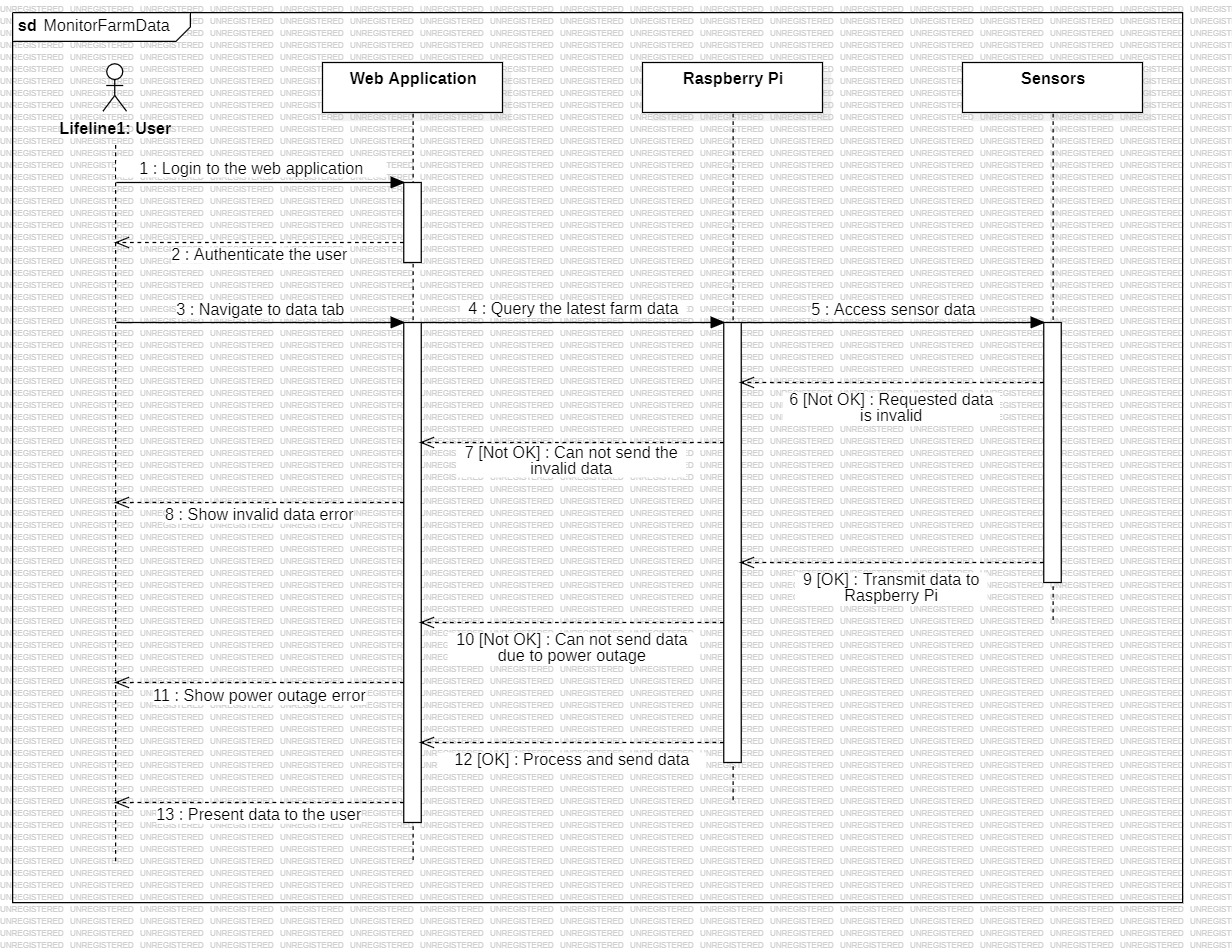
\includegraphics[width=1\linewidth]{Figures/monitor_farm_data_sequence_diagram.jpg}
        \caption{Sequence Diagram for \textbf{Monitor Farm Data} Use Case}
        \label{MonitorFarmDataSequenceDiagram}
\end{figure}

\newpage

% View System Logs Use Case Table
\begin{longtblr}
[
 caption = {Tabular Description of the \textbf{View System Logs} Use Case},
 label = {ViewSystemLogs}
]
{
  colspec = {|X|X|},
  hlines
}
\textbf{Use Case Name} & View System Logs \\ \hline
\textbf{Actors} & System Admin \\ \hline
\textbf{Description} & System Admins access and review the system log to monitor FarmBot's software activities, operational history, and system alerts. \\ \hline
\textbf{Preconditions} & The System Admin must have administrative credentials. Log files must be stored. \\ \hline
\textbf{Data} & Log entries containing information about system operations, errors, user activities, and hardware statuses. \\ \hline
\textbf{Response} & Display of system logs. \\ \hline
\textbf{Stimulus} & One of the system admins attempts to view system logs. \\ \hline
\textbf{Normal Flow} & {
	1. System Admin logs into the FarmBot Web Server with administrative credentials.\\
	2. System admin access log files on the server.
}
\\ \hline
\textbf{Alternative Flow} & - \\ \hline
\textbf{Exception Flow} & - \\ \hline
\textbf{Post Conditions} & System log records in the log files must be displayed to the admin. \\ \hline
\textbf{Comments} & This use case is essential for system maintenance and troubleshooting, allowing the System Admin to identify and address issues proactively.
\end{longtblr}

% View Financial Analysis Pane Use Case Table
\begin{longtblr}
[
 caption = {Tabular Description of the \textbf{View Financial Analysis Pane} Use Case},
 label = {ViewFinancialAnalysisPane}
]
{
  colspec = {|X|X|},
  hlines
}
\textbf{Use Case Name} & View Financial Analysis Pane \\ \hline
\textbf{Actors} & User, Web Application \\ \hline
\textbf{Description} & Users access the Financial Analysis Pane within the FarmBot Web Application to review financial data related to their farming operations. \\ \hline
\textbf{Preconditions} & The user must be logged into the FarmBot Web Application. \\ \hline
\textbf{Data} & Financial data including costs of resources (water, seeds, fertilizers, etc.), operational expenses, and projected revenues from crop yields. \\ \hline
\textbf{Response} & Display of financial analysis and projections in a graphical or tabulated format. \\ \hline
\textbf{Stimulus} & The user selects the Financial Analysis Pane from the Web Application's dashboard. \\ \hline
\textbf{Normal Flow} & {
	1. User navigates to and selects the Financial Analysis Pane option.\\
	2. System Admin makes desired changes to the settings and submits the modifications.\\
	3. The Web Application retrieves and displays financial data related to the user’s farm.\\
	4. User reviews the information for planning and decision-making purposes.
}
\\ \hline
\textbf{Alternative Flow} & - \\ \hline
\textbf{Exception Flow} & If financial data cannot be retrieved, an error message is displayed. \\ \hline
\textbf{Post Conditions} &  The user has accessed and reviewed the financial analysis of their farming operations. \\ \hline
\textbf{Comments} & This use case is vital for users to understand the financial performance of their farm, enabling better resource management, operational planning, and profitability analysis.
\end{longtblr}

% View Hardware Information Use Case Table
\begin{longtblr}
[
 caption = {Tabular Description of the \textbf{View Hardware Information} Use Case},
 label = {ViewHardwareInformation}
]
{
  colspec = {|X|X|},
  hlines
}
\textbf{Use Case Name} & View Hardware Information \\ \hline
\textbf{Actors} & User, Web Application \\ \hline
\textbf{Description} & Users access a dedicated pane within the FarmBot Web Application to view and manage information about their FarmBot's hardware and tooling \\ \hline
\textbf{Preconditions} & The user must be logged into the FarmBot Web Application. \\ \hline
\textbf{Data} & Details on installed hardware components (tracks, gantry, tool mounts, sensors), their status, and configuration settings including dimensions and operational status (active/inactive). \\ \hline
\textbf{Response} & The Web Application displays the hardware information pane, allowing users to view, modify, and update their hardware configurations. \\ \hline
\textbf{Stimulus} & The user selects the hardware information option in the Web Application. \\ \hline
\textbf{Normal Flow} & {
	1. User navigates to the hardware information pane using the dropdown menus.\\
	2. The pane displays current hardware configurations, with options to add new components or modify existing ones.\\
	3. Users can activate or deactivate specific hardware components, adjust dimensions, or update the system with new hardware additions.
}
\\ \hline
\textbf{Alternative Flow} & - \\ \hline
\textbf{Exception Flow} & If there's an issue accessing or modifying hardware data, an error message is displayed. \\ \hline
\textbf{Post Conditions} & The user has successfully accessed and possibly modified the hardware information for their FarmBot. \\ \hline
\textbf{Comments} & This use case facilitates effective management and customization of FarmBot's hardware setup, enabling users to optimize their system according to specific farming needs and space requirements.
\end{longtblr}

% View Resource Usage Use Case Table
\begin{longtblr}
[
 caption = {Tabular Description of the \textbf{View Resource Usage} Use Case},
 label = {ViewResourceUsage}
]
{
  colspec = {|X|X|},
  hlines
}
\textbf{Use Case Name} & View Resource Usage\\ \hline
\textbf{Actors} & User, Web Application\\ \hline
\textbf{Description} &  Users access the Resource Usage Pane within the FarmBot Web Application to examine the consumption and costs of resources such as electricity, water, seeds, and fertilizers.\\ \hline
\textbf{Preconditions} & The user must be logged into the FarmBot Web Application.\\ \hline
\textbf{Data} & Historical, current, and projected resource usage data, including volume, timing, and monetary costs.\\ \hline
\textbf{Response} & Display of an interactive graph showing resource usage with zoom and filter capabilities for detailed analysis.\\ \hline
\textbf{Stimulus} & The user selects the Resource Usage Pane from within the Web Application.\\ \hline
\textbf{Normal Flow} & {
	1. User navigates to and selects the Resource Usage Pane.\\
	2. The Web Application presents an interactive graph detailing resource usage.\\
	3. User interacts with the graph to zoom in on details or filter by specific resources like water usage on tomatoes.
}
\\ \hline
\textbf{Alternative Flow} & -\\ \hline
\textbf{Exception Flow} & If data cannot be retrieved, an error message is displayed.\\ \hline
\textbf{Post Conditions} & The user has accessed detailed resource usage information, aiding in efficient management and cost-saving strategies.\\ \hline
\textbf{Comments} & This feature enables users to closely monitor and optimize resource consumption, contributing to sustainable and cost-effective farm management.
\end{longtblr}

% View System Information Use Case Table
\begin{longtblr}
[
 caption = {Tabular Description of the \textbf{View System Information} Use Case},
 label = {ViewSystemInformation}
]
{
  colspec = {|X|X|},
  hlines
}
\textbf{Use Case Name} & View System Information\\ \hline
\textbf{Actors} & User, Web Application\\ \hline
\textbf{Description} & Users access the System Information Pane within the FarmBot Web Application to review detailed information about their FarmBot system's status.\\ \hline
\textbf{Preconditions} & The user must be logged into the FarmBot Web Application.\\ \hline
\textbf{Data} & System status data, manual control options, financial expenditures on inputs, expected revenues from crops, and other operational factors such as maintenance and logistics costs.\\ \hline
\textbf{Response} & The Web Application displays the system information with the capability for users to apply advanced filtering to the data presented.\\ \hline
\textbf{Stimulus} & The user selects the System Information Pane from the Web Application's dashboard.\\ \hline
\textbf{Normal Flow} & {
	1. User navigates to and selects the System Information Pane option.\\
	2. The Web Application retrieves and displays the current system information.\\
	3. User interacts with the pane to view specific system details, utilizing filtering options as needed for detailed analysis.
}
\\ \hline
\textbf{Alternative Flow} & -\\ \hline
\textbf{Exception Flow} & If data cannot be retrieved, an error message is displayed.\\ \hline
\textbf{Post Conditions} & The user has accessed and reviewed the system status and financial analysis of their farming operations.\\ \hline
\textbf{Comments} & This use case provides users with crucial information for understanding their FarmBot's operational status and the financial health of their farm, facilitating informed decision-making and system management.
\end{longtblr}

% Store Farm Data Use Case Table
\begin{longtblr}
[
 caption = {Tabular Description of the \textbf{Store Farm Data} Use Case},
 label = {StoreFarmData}
]
{
  colspec = {|X|X|},
  hlines
}
\textbf{Use Case Name} & Store Farm Data\\ \hline
\textbf{Actors} & User, OpenFarm.cc API\\ \hline
\textbf{Description} & Users upload and store their farm data on OpenFarm.cc, enabling them to share their experiences and leverage data shared by others for optimizing their FarmBot operations.\\ \hline
\textbf{Preconditions} & The user must be registered with OpenFarm.cc and have an active internet connection.\\ \hline
\textbf{Data} & Farm layouts, plant growth data, operational sequences, and other relevant farming data.\\ \hline
\textbf{Response} & The data is successfully uploaded and stored on OpenFarm.cc, making it accessible to other users.\\ \hline
\textbf{Stimulus} & The user selects the option to upload data to OpenFarm.cc through the FarmBot Web Application.\\ \hline
\textbf{Normal Flow} & {
	1. User is prompted to log in or verify their OpenFarm.cc account if not already authenticated.\\
  2. User selects the option to store farm data on OpenFarm.cc.\\
  3. User selects or inputs the farm data they wish to upload.\\
  4. The Web Application sends the data to OpenFarm.cc using its API.\\
  5. OpenFarm.cc confirms successful data storage.\\
  6. The user receives confirmation of the successful upload within the FarmBot Web Application.
}
\\ \hline
\textbf{Alternative Flow} & -\\ \hline
\textbf{Exception Flow} & If there's an issue with internet connectivity or OpenFarm.cc API is unavailable, the user is informed of the failure to store data. If authentication fails, the user is prompted to re-authenticate.\\ \hline
\textbf{Post Conditions} & The user's farm data is stored on OpenFarm.cc, available for their personal use and sharing with the community.\\ \hline
\textbf{Comments} & This use case expands the utility of FarmBot by integrating community-driven data sharing, offering users a platform to contribute to and benefit from collective farming knowledge and data.
\end{longtblr}

% Store Farm Data State Diagram
\begin{figure}[htbp]
  \centering
  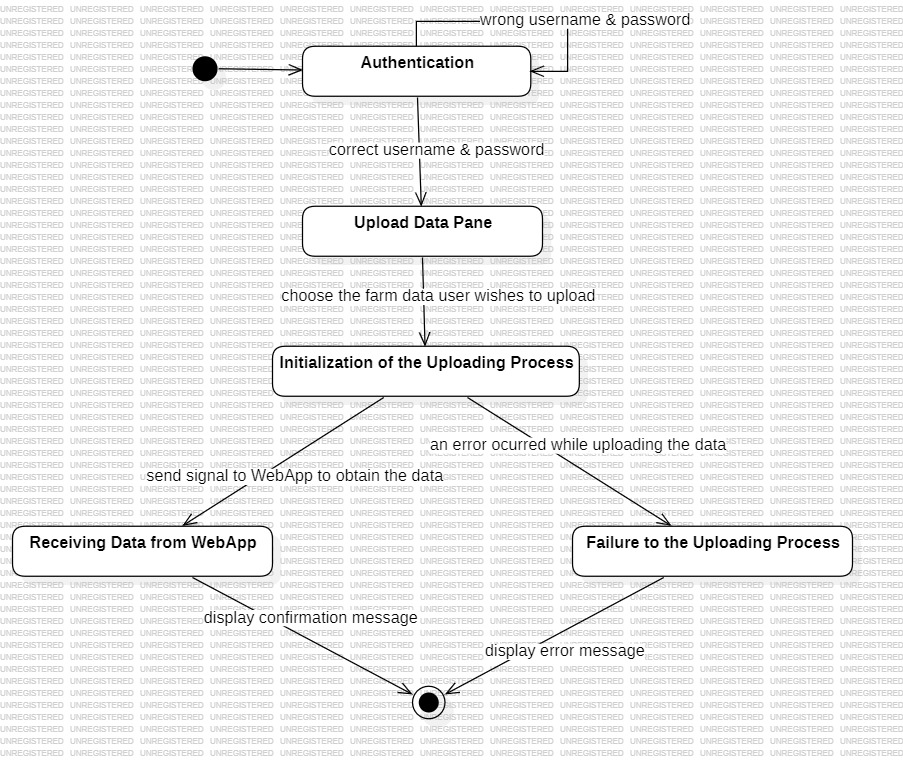
\includegraphics[width=1\linewidth]{Figures/store_farm_data_state_diagram.jpg}
  \caption{State Diagram for \textbf{Store Farm Data} Use Case}
  \label{StateDiagram}
\end{figure}

\newpage

\section{Logical Database Requirements}
\begin{figure}[htbp]
        \centering
        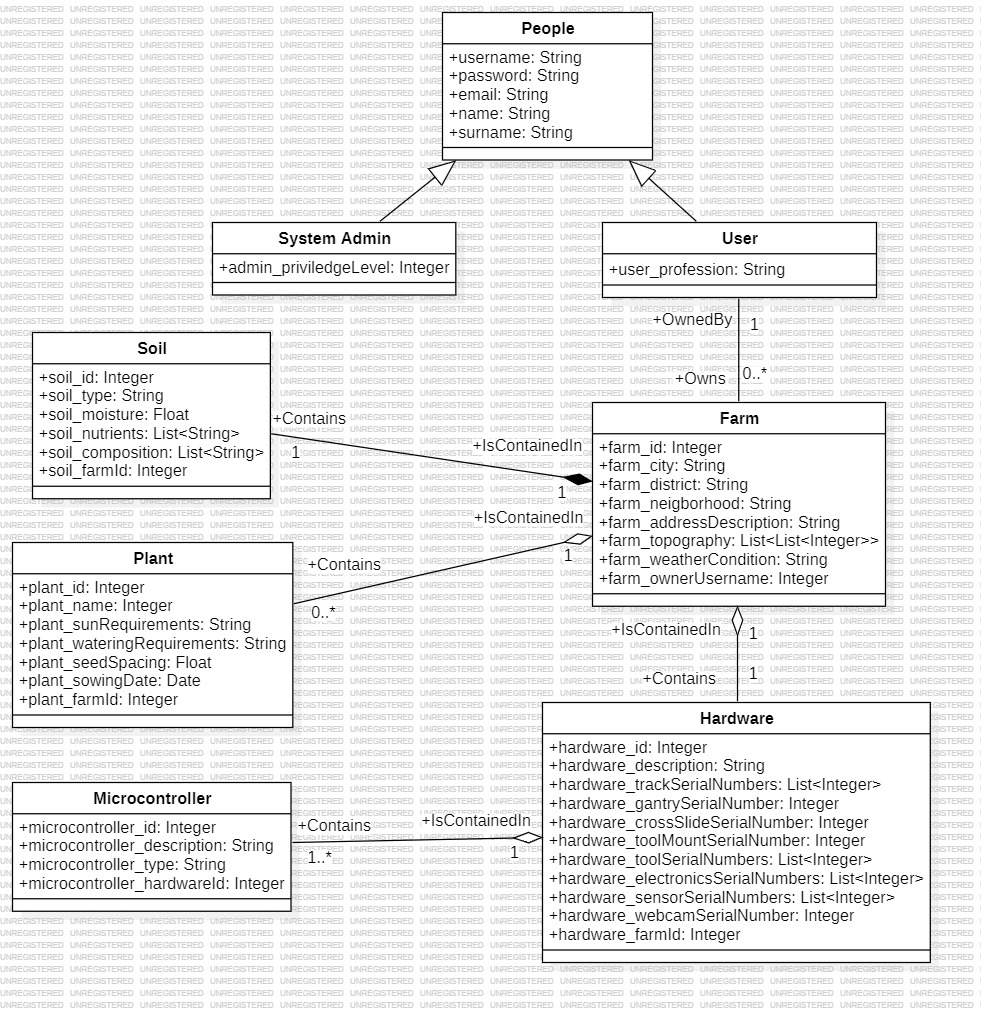
\includegraphics[width=1\linewidth]{Figures/logical_database_diagram.jpg}
        \caption{Logical Database Diagram}
        \label{LogicalDatabaseDiagram}
\end{figure}

\newpage

\section{Design Constraints}
\begin{itemize}
    \item FarmBot must adhere to international data privacy laws like GDPR, ensuring user data is handled according to legal standards.
    \item Its development must align with the open-source licenses like MIT of its hardware and software components, maintaining public accessibility and respecting intellectual property rights.
    \item Compliance with electrical and mechanical safety standards is crucial to prevent user injury or crop damage.
    \item FarmBot should integrate into various farming operations without harming soil quality or the ecosystem, adaptable to different farming scales.
    \item Requires industry-standard data exchange and system integration protocols to ensure compatibility with existing agricultural technology and cloud services.
\end{itemize}
These constraints guide FarmBot's development, focusing on safety and effectiveness while meeting legal and environmental standards.

\section{System Quality Attributes}
\begin{itemize}
    \item \textbf{Reliability:} FarmBot requires a highly reliable software system to ensure accurate and timely execution of farming tasks. This includes:
    \begin{itemize}
        \item Regular backup of farm data, including designs, user settings, and operational logs, to prevent data loss.
        \item Zero tolerance for operational errors that could impact plant health or resource use efficiency.
    \end{itemize}
    \item \textbf{Availability:} The FarmBot system is designed for high availability to support continuous agricultural activities. The cloud-based services of FarmBot should ensure data synchronization and system updates without interrupting core functionalities.
    \item \textbf{Security:} Protecting user data and ensuring the integrity of FarmBot operations is essential:
    \begin{itemize}
        \item Maintain access logs for monitoring and auditing purposes.
        \item Implement role-based access controls to segregate user functionalities and protect sensitive system settings.
        \item Enforce data integrity checks for critical variables to prevent unauthorized modifications.
        \item Ensure privacy of user data in compliance with data protection regulations.
    \end{itemize}
    \item \textbf{Maintainability:} The software architecture of FarmBot emphasizes maintainability to facilitate updates and enhancements:
    \begin{itemize}
        \item Adhere to modularity in design to simplify updates and module replacements.
        \item Adopt continuous integration and deployment practices to streamline software updates and patch implementations.
    \end{itemize}
    \item \textbf{Portability:} FarmBot software aims to be easily portable to support a wide range of hardware setups and operating environments. It has software designed to be compatible with major operating systems and platforms, including Linux-based systems for Raspberry Pi and web browsers for the WebApp.
\end{itemize}

\section{Supporting Information}
The FarmBot project is an open-source initiative focused on advancing agricultural practices through automation and technology. The entire source code and design files for both the hardware and software components are accessible on GitHub, allowing anyone interested to view, analyze, and contribute to the project's development. Numerous open issues on the GitHub page are awaiting solutions, offering opportunities for contributors to engage in problem-solving and feature enhancement.\\\\
Beyond software development, there are additional ways to support FarmBot. Enthusiasts and professionals can contribute by sharing insights on optimal farming practices, suggesting improvements for hardware design, or even participating in educational outreach to spread knowledge about this technology. By joining the FarmBot community, you contribute to a global movement aimed at making sustainable farming accessible to everyone, leveraging the collective knowledge and skills of a diverse group of contributors.

